\begin{beginningnote}
    Si tenga presente che alcuni termini utilizzati nel documento riportano la lettera \textbf{G} in apice, allo scopo di evidenziare le parole che assumono uno specifico 
    significato nell'ambito del progetto. Per comprenderle in maniera corretta, si rimanda il lettore al documento ``Glossario", che contiene un elenco completo di tutte le 
    terminologie utilizzate con relative definizioni, allo scopo di costruire un linguaggio uniforme che possa migliorare la comunicazione tra i componenti interni al gruppo 
    e gli stakeholder\textsuperscript{G} esterni.
\end{beginningnote}

%%%%%%%%%%%%%%%%%%%%%%%%%%%%%%%%%%%
% SCOPO DEL DOCUMENTO
%%%%%%%%%%%%%%%%%%%%%%%%%%%%%%%%%%%
\section{Scopo del documento}\label{sec:scopo_del_documento}
    Lo scopo del seguente documento è quello di illustrare le funzionalità fornite dall'applicazione e fornire agli utenti le istruzioni necessarie per il corretto utilizzo 
    della stessa. Si intende quindi informare ogni utilizzatore sui requisiti minimi necessari per la corretta esecuzione dell'applicativo al fine di fornire un'esperienza 
    utente chiara ed esaustiva.    

%%%%%%%%%%%%%%%%%%%%%%%%%%%%%%%%%%%
% SCOPO DEL PROGETTO
%%%%%%%%%%%%%%%%%%%%%%%%%%%%%%%%%%%
\section{Scopo del progetto}\label{sec:scopo_del_progetto}

    Il progetto nasce nell'ambito dei \textbf{sistemi gestionali di magazzino}, meglio noti con il termine inglese di \textit{Warehouse Management Systems} (WMS), con 
    l'obiettivo di risolvere una serie di problematiche derivanti dalle soluzioni tradizionali tuttora presenti sul mercato.\\
    Il focus principale sarà migliorare la user experience, tramite la realizzazione di un applicativo che proponga all'utente un'interazione con il magazzino in un 
    ambiente di lavoro 3D. \\
    Tale soluzione, rispetto ai tradizionali sistemi 2D, garantirebbe una maggiore comprensione degli spazi, proponendo una visualizzazione più intuitiva e completa 
    degli spazi di magazzino. Permetterebbe quindi all'utente di prendere decisioni in modo più efficace ed efficiente, permettendo così di ottimizzare i processi di logistica.

    Per raggiungere questo obiettivo, l'ambiente di lavoro non può essere una semplice visualizzazione del magazzino. L'utente dovrà infatti poter:
    \begin{itemize}
        \item Spostarsi all'interno dell'ambiente 3D;
        \item Progettare le scaffalature che sono presenti nel magazzino e modificarle nel tempo;
        \item Simulare i flussi di movimento di prodotti.
    \end{itemize}

    Il progetto deve concretizzarsi nella realizzazione di una web app fruibile agli impiegati d'ufficio ed incentrata sulla visualizzazione 3D del magazzino.
    Per visionare il capitolato\textsuperscript{G} completo e la documentazione del gruppo, si veda la sezione \hyperref[sec:riferimenti_esterni]{Riferimenti Esterni} 
    del documento.

\newpage


%%%%%%%%%%%%%%%%%%%%%%%%%%%%%%%%%%%
% REQUISITI E COMPATIBILITA'
%%%%%%%%%%%%%%%%%%%%%%%%%%%%%%%%%%%
\section{Requisiti e compatibilità}\label{sec:requisiti_e_compatibilità}
    In questa sezione sono illustrati i requisiti minimi neccessari per una corretta esecuzione dell'applicativo realizzato. Saranno quindi evidenziate le caratteristiche 
    che ogni terminale deve soddisfare per configurare correttamente l'ambiente di esecuzione.

    \subsection{Requisiti software}\label{sec:requisiti_e_compatibilità:software}
    L'applicativo sarà reso disponibile all'utente attraverso due modalità: la \textit{modalità utente}\textsuperscript{G} e la \textit{modalità programmatore}\textsuperscript{G}.\\
    La \textit{modalità programmatore}\textsuperscript{G} è consigliata solamente ad utilizzatori esperti. \\
    Per questa esecuzione saranno necessari: l'installazione del software Node.js, alla versione 20.0 o superiore, e un browser stabile. \\
    Per una corretta installazione del software si rimanda alla pagina dedicata, presente nella sezione \hyperref[sec:riferimenti_esterni]{Riferimenti Esterni} del documento. 
    L'applicativo è stato testato per il corretto funzionamento con i principali motori di ricerca che si riportano qui sotto:
    \begin{xltabular}{\textwidth}{ X | X}

        \rowcolor{black}
        \textbf{\color{white} Motore di ricerca} & \textbf{\color{white} Verisone}\\ 
        \hline
        \endhead

        Google Chrome & 124.0 \\
        \hline

        Micorsoft Edge & 124.0 \\
        \hline
        
        Safari & 17.0 \\
        \hline

        Mozilla Firefox & 115.0 \\
        \hline

        Opera & 109.0 \\
        \hline
        
        \caption{Tabella dei requisiti software}
        \label{tab:requisiti:soft}
    \end{xltabular}
    \noindent La \textit{modalità programmatore}\textsuperscript{G} è invece accessibile anche da utenti meno esperti. Non necessita di particolari configurazioni ma si raccomanda 
    comunque di utilizzare uno dei browser sopra citati. \\



    \subsection{Requisiti hardware}\label{sec:requisiti_e_compatibilità:hardware}
    L'applicativo realizzato appartiene alla categoria delle web-app. L'esecuzione non avviene quindi in locale sul terminale utilizzato ma viene effettuata direttamente dal 
    browser scelto dall'utente. Non sono quindi richieste dei particolari requisiti hardware minimi per l'esecuzione.\\
    Viene comunque consigliato l'utilizzo di un terminale aggiornato che, a titolo di riferimento, può essere identificato in:
    \begin{xltabular}{\textwidth}{ X | X}

        \rowcolor{black}
        \textbf{\color{white} Componente} & \textbf{\color{white} Requisito minimo consigliato}\\ 
        \hline
        \endhead
        
        Connessione Internet & Connessione Internet stabile e veloce \\
        \hline

        Processore & Quad-Core 1,80 GHz \\
        \hline
        
        Memoria RAM & 8GB DDR3 \\
        \hline

        \caption{Tabella dei requisiti hardware}
        \label{tab:requisiti:hard}
    \end{xltabular}

    \newpage

    

%%%%%%%%%%%%%%%%%%%%%%%%%%%%%%%%%%%
% INSTALLAZIONE ED ESECUZIONE
%%%%%%%%%%%%%%%%%%%%%%%%%%%%%%%%%%%
\section{Installazione ed esecuzione}\label{sec:install_run}

    L'esecuzione dell'applicazione si differisce in base alla modalità di esecuzione scelte. Pertanto si riportano separatamente le due modalità disponibili. \\
    \textbf{In caso si scelga di eseguire il programma in \textit{modalità utente}\textsuperscript{G} è possibile trascurare la sezione installazione. Si rimanda quindi alla 
    sezione \hyperref[sec:install_run:user]{esecuzione della modalità utente}.} \\ 

    \subsection{Modalità programmatore}\label{sec:install_run:esperto}
    Questa sezione intende definire le operazioni di installazione preliminari necessarie per l'esecuzione dell'applicativo in \textit{modalità programmatore}\textsuperscript{G}.\\
    Di seguito saranno quindi elencati i passaggi necessari per la clonazione della repository e l'avvio dell'applicazione. \\
    
    \subsubsection{Clonazione della repository}\label{sec:install_run:esperto:clone}
    Per scaricare tutti i file neccessari all'esecuzione è possibile: 
    \begin{enumerate}
        \item Scaricare il codice (archivio in formato \textit{.zip}) direttamente dal seguente link: \\  
        \url{INSERIRE LINK CORRETTO} \textcolor{gray}{\textit{(ultimo accesso 04-05-24)}}
        \item Utilizzare i servizi messi a disposizione dal software Git, che deve essere installato sulla macchina di esecuzione
        \begin{itemize}
            \item Posizionarsi sulla repository di interesse.
            \item Utilizzare il comando:\\
            \textbf{git clone \url{INSERIRE LINK CORRETTO} }
        \end{itemize}
    \end{enumerate}

    \subsubsection{Avvio dell'applicativo}\label{sec:install_run:esperto:avvio}
    Una volta creata una copia del codice in una repository locale del terminale posizionarsi all'interno di essa in corrispondenza della repository \textit{Diamociunnome}.\\
    Sarà quindi neccessaio aprire un terminale in corrispondenza di tale repository ed eseguire i seguenti passaggi: 
    \begin{enumerate}
        \item Installare le dipendenze (necessario solamente al primo avvio): \\  
        \textbf{npm install}
        \item Buildare l'applicazione con il comando: \\  
        \textbf{npm run dev}
        \item Una volta terminata la fase di built dell'applicativo, aprire un browser e ricercare la seguente pagina web: \\  
        \url{http://localhost:3000}
    \end{enumerate}

    \subsection{Modalità utente}\label{sec:install_run:user}
    Come già spiegato in \textit{modalità utente}\textsuperscript{G} non sarà necessaria alcuna procedura preliminare. L'utente dovrà solamente collegarsi al seguente link per poter eseguire 
    direttamente la web-app dal proprio browser predefinito: 
    \begin{itemize}
        \item\url{inserire il link corretto}
    \end{itemize}

    \newpage



    
%%%%%%%%%%%%%%%%%%%%%%%%%%%%%%%%%%%
% ISTRUZIONI D'USO 
%%%%%%%%%%%%%%%%%%%%%%%%%%%%%%%%%%%
\section{Istruzioni d'uso}\label{sec:Istruzioni_uso}

    \subsection{Configurazione magazzino}\label{sec:creazione}
        Nell'applicativo realizzato non è necessaria alcuna login iniziale. L'applicativo si presenta quindi subito con la schermata iniziale in cui l'utente è 
        invitato ad inserire tutti i dati necessari per poter configurare o caricare il magazzino da visualizzare.
        \begin{figure}[h!]
            \centering
            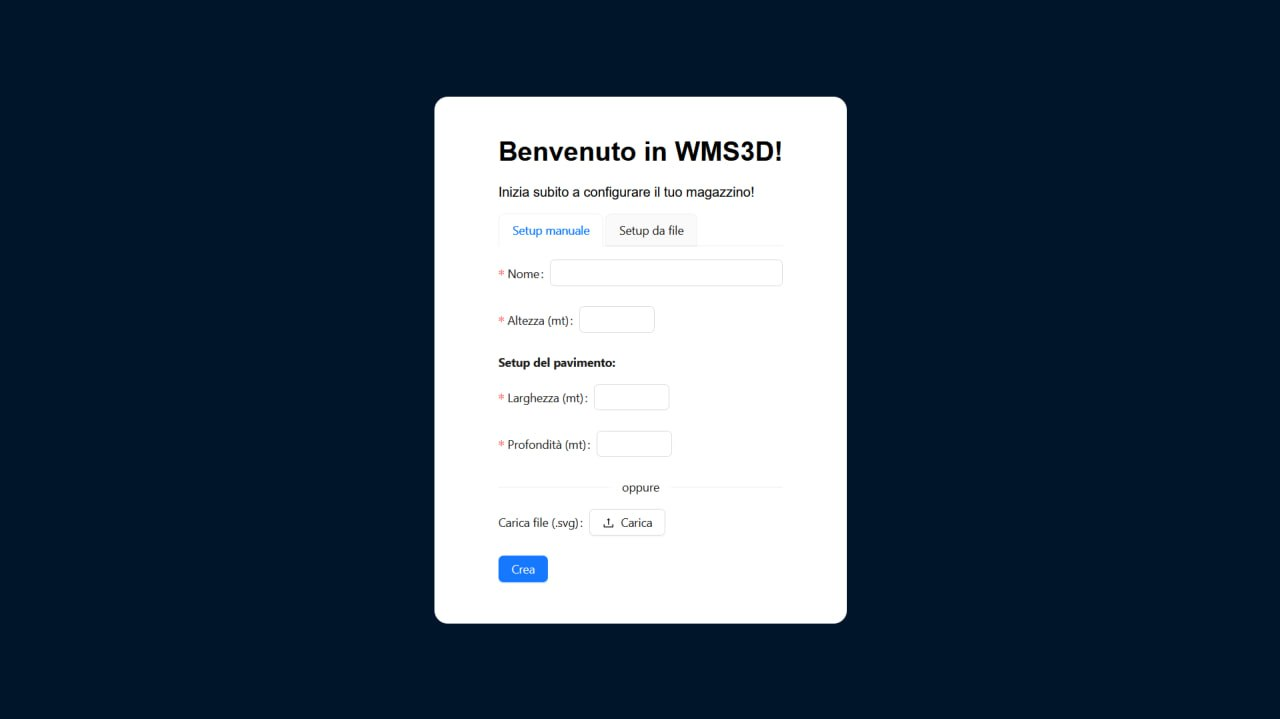
\includegraphics[width=0.8\textwidth]{images/schermata_iniziale.png}
            \caption{Schermata iniziale di configurazione}
        \end{figure}\\
        \noindent In questa sezione l'utente avrà la facoltà di scegliere se configurare manualmente il magazzino o, in alternativa, caricare un layout già pronto all'uso.

        
        \subsubsection{Configurazione manuale del magazzino}\label{sec:creazione:configurazione}
            Se la scelta ricade sulla configurazione manuale del magazzino l'utente dovrà inserire nell'apposito form i seguenti dati: 
            \begin{itemize}
                \item Un nome da assegnare al magazzino
                \item L'altezza (espressa in metri) del magazzino
                \item La pianta del magazzino. Per tale configurazione sono possibili due alternative:
                \begin{enumerate}
                    \item Impostare una semplice pianta rettangolare, andando a indicare le misure di larghezza e profondità (sempre espresse in metri)
                    \item Caricare una pianta personalizzata, andando a caricare un file .svg appositamente realizzato. 
                \end{enumerate}
            \end{itemize}
            Durante l'inserimento di ciascun campo, sia numerico che testuale, l'utente sarà aiutato dal sistema al fine di inserire correttamente i dati richiesti.\\
            Sarà infatti assistito durante la fase di inserimento degli input in modo tale da garantire una corretta configurazione iniziale del magazzino.
            \paragraph{Caricamento pianta da file .svg} \label{sec:creazione:configurazione:svg}
            Attraverso tale funzionalità l'utente avrà modo di caricare un layout predefinito e salvato in un apposito file .svg.\\
            --------------\\
            --------------\\
            --------------\\
            NB: aggiungere le caratteristiche del file svg\\
            --------------\\
            --------------\\
            --------------\\
            Anche in questo caso il caricamento di un file non conforme (non .svg) verrà gestito dal sistema che ritornerà un messaggio di errore e permetterà 
            all'utente di rieseguire l'operazione. 
            \begin{figure}[h!]
                \centering
                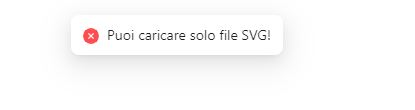
\includegraphics[]{images/errore_caricamento_svg.png}
                \caption{Configurazione magazzino: Errore caricamento .svg}
            \end{figure}
           

        
        \subsubsection{Caricamento del magazzino}\label{sec:creazione:caricamento}
            Nel caso in cui l'utente abbia già realizzato un render 3D del magazzino avrà la possibilità di ricaricare quanto già realizzato grazie all'apposita sezione. 
            \begin{figure}[h!]
                \centering
                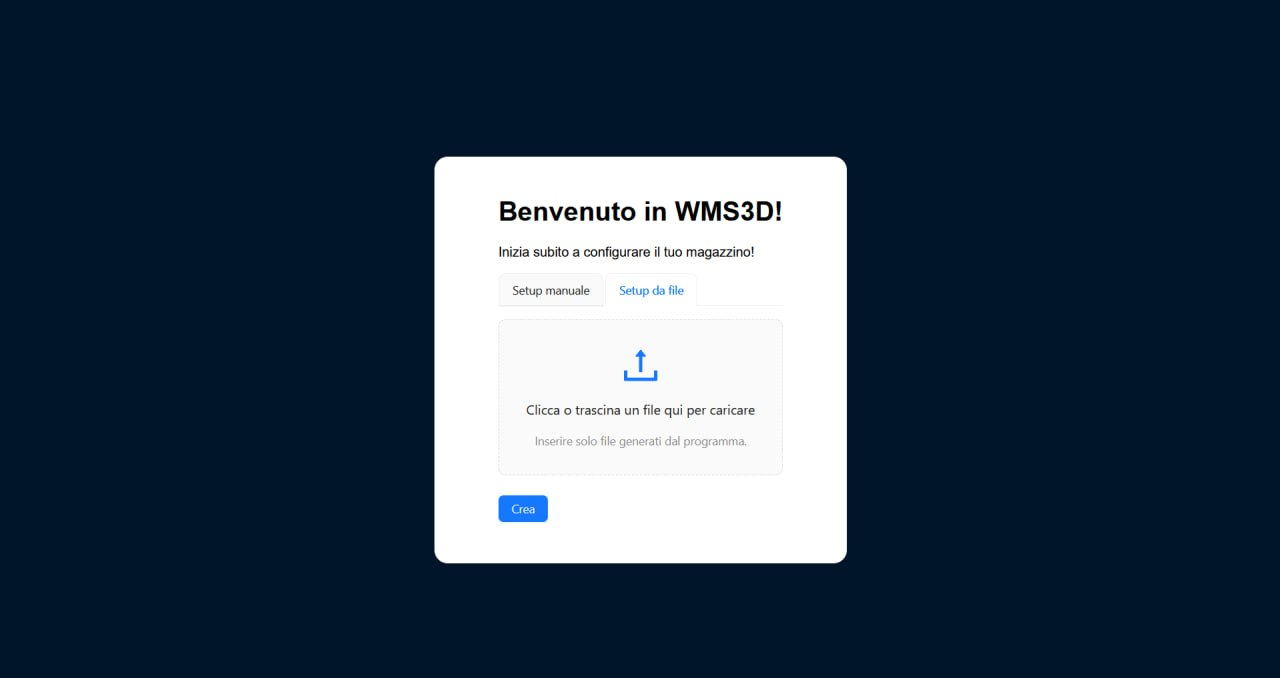
\includegraphics[width=0.8\textwidth]{images/caricamento.png}
                \caption{Sezione di caricamento da file .json}
            \end{figure}\\
            \noindent Così come per il caricamento della pianta da .svg, anche in questo caso sarà il sistema a verificare la correttezza del tipo di file che si sta cercando 
            di importare. \\
            --------------\\
            --------------\\
            --------------\\
            NB: aggiungere le caratteristiche del file json\\
            --------------\\
            --------------\\
            --------------\\
    \newpage        

    \subsection{Magazzino configurato}\label{sec:principale}
        Una volta configurato correttamente il magazzino l'utente si troverà di fronte alla pagina principale dell'applicativo. 
        In questa pagina troverà: 
        \begin{itemize}
            \item Una sezione a sinistra di supporto all'utente, la \textbf{libreria}\textsuperscript{G}. La libreria, in quanto di solo supporto all'utente, è 
                  oscurabile, tramite l'apposito tasto presente nella barra di navigazione. 
            \item Una barra di navigazione, contenente da due tasti: il tasto per oscurare la libreria a sinista e il tasto per il salvataggio a destra. 
                  Attraverso quest'ultimo bottone verrà infatti lanciato il download di un file .json contentente tutte le informazioni in merito 
                  al magazzino finora creato. In questo modo sarà possibile salvare su file lo stato di fatto del magazzino. 
            \item La sezione 3D nella quale viene renderizzato il magazzino appena creato. In essa troveremo quindi una rappresentazione di uno spazio tridimensionale 
                  all'interno del quale si potranno distinguere: 
            \begin{enumerate}
                \item Una superficie bianca piana suddivisa in blocchi quadrati di egual misura, corrispondenti a un metro quadrato
                \item Una porzione del piano sopra citato evidenziato in giallo, a rappresentare la pianta del magazzino appena configurato o caricato
                \item Delle superfici grigio chiaro, che si sviluppano dalla porzione di piano evidenziata, che rappresentano i muri del magazzino e quindi forniscono 
                l'informazione relativa all'altezza del magazzino
            \end{enumerate}
        \end{itemize}
        \begin{figure}[h!]
            \centering
            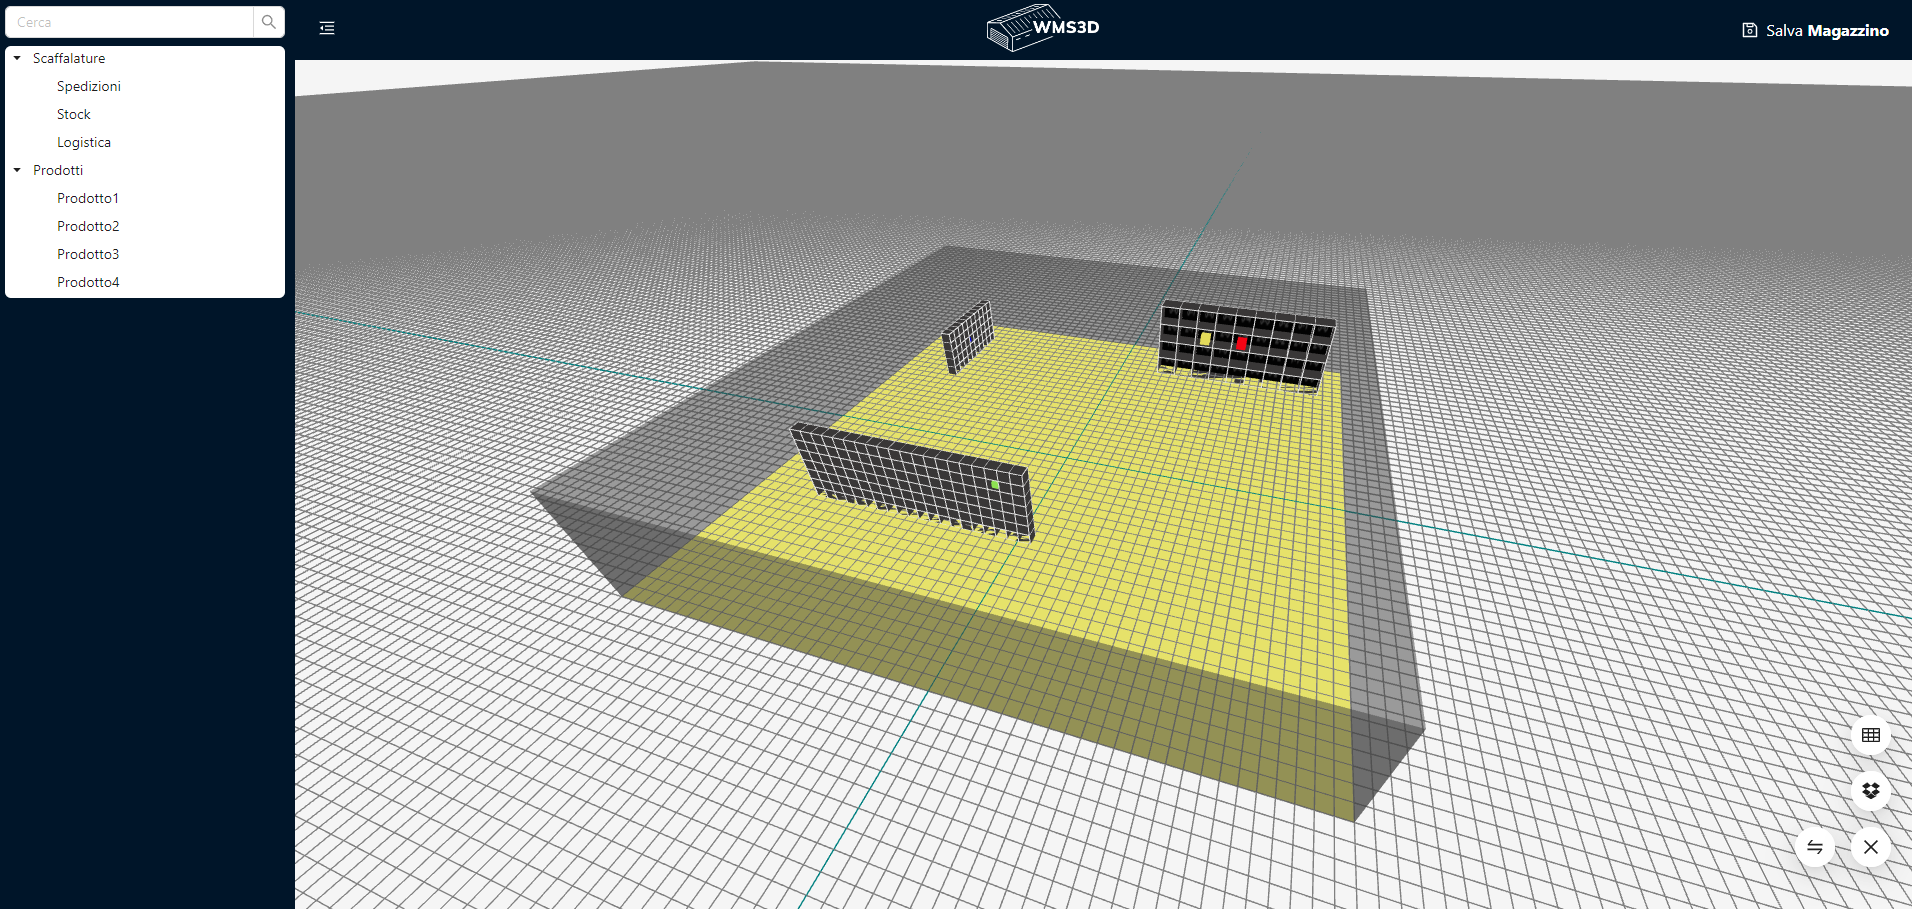
\includegraphics[width=0.8\textwidth]{images/schermata_principale.png}
            \caption{Schermata principale dell'applicativo}
        \end{figure}

    
        \subsubsection{Esplorazione e ricerca}\label{sec:principale:esplorare}
            \paragraph{Navigazione all'interno del render 3D} \label{sec:principale:esplorare:navigare}
                All'interno della sezione 3D l'utente avrà modo, attraverso la navigazione tramite mouse o tastiera, di potersi spostare all'interno della rappresentazione 3D.
                Supponendo un utilizzo da parte di un mouse a tre tasti: il tasto destro, il tasto sinistro e il tasto centrale, o rotella, l'utilizzatore avrà la 
                possibilità di effettuare uno zoom in/out attraverso il tasto centrale mentre grazie ai tasti destro e sinistro sarà in grado di cambiare
                l'angolazione e le prospettive di visualizzazione. \\
                Sono garantiti anche alcuni comandi da tastiera: 
                \begin{itemize}
                    \item \textbf{Tasto W}: zoom in
                    \item \textbf{Tasto S}: zomm out
                    \item \textbf{Tasto D}: spostamento verso destra
                    \item \textbf{Tasto A}: spostamento verso sinistra
                \end{itemize}
                L'utente avrà quindi modo di mouversi liberamente all'interno del render 3D, mantendendo però il focus sul magazzino ed il suo contenuto. \\
                Sarà inoltre in grado di selezionare scaffalature e bin in modo da le scaffalature e i bin presenti nel render.\\
                Una volta selezionato un componente comparirà un piccolo riquadro, in alto a destra, in grado di fornire le informazioni sull'oggetto selezionato e, 
                in aggiunta, verrà rimarcato il componente selezionato anche all'interno della libreria. \\
                In caso di selezione scaffalatura verranno quindi visualizzate le caratteristiche di capacità e configurazione della scaffalatura stessa. 
                \begin{figure}[h!]
                    \centering
                    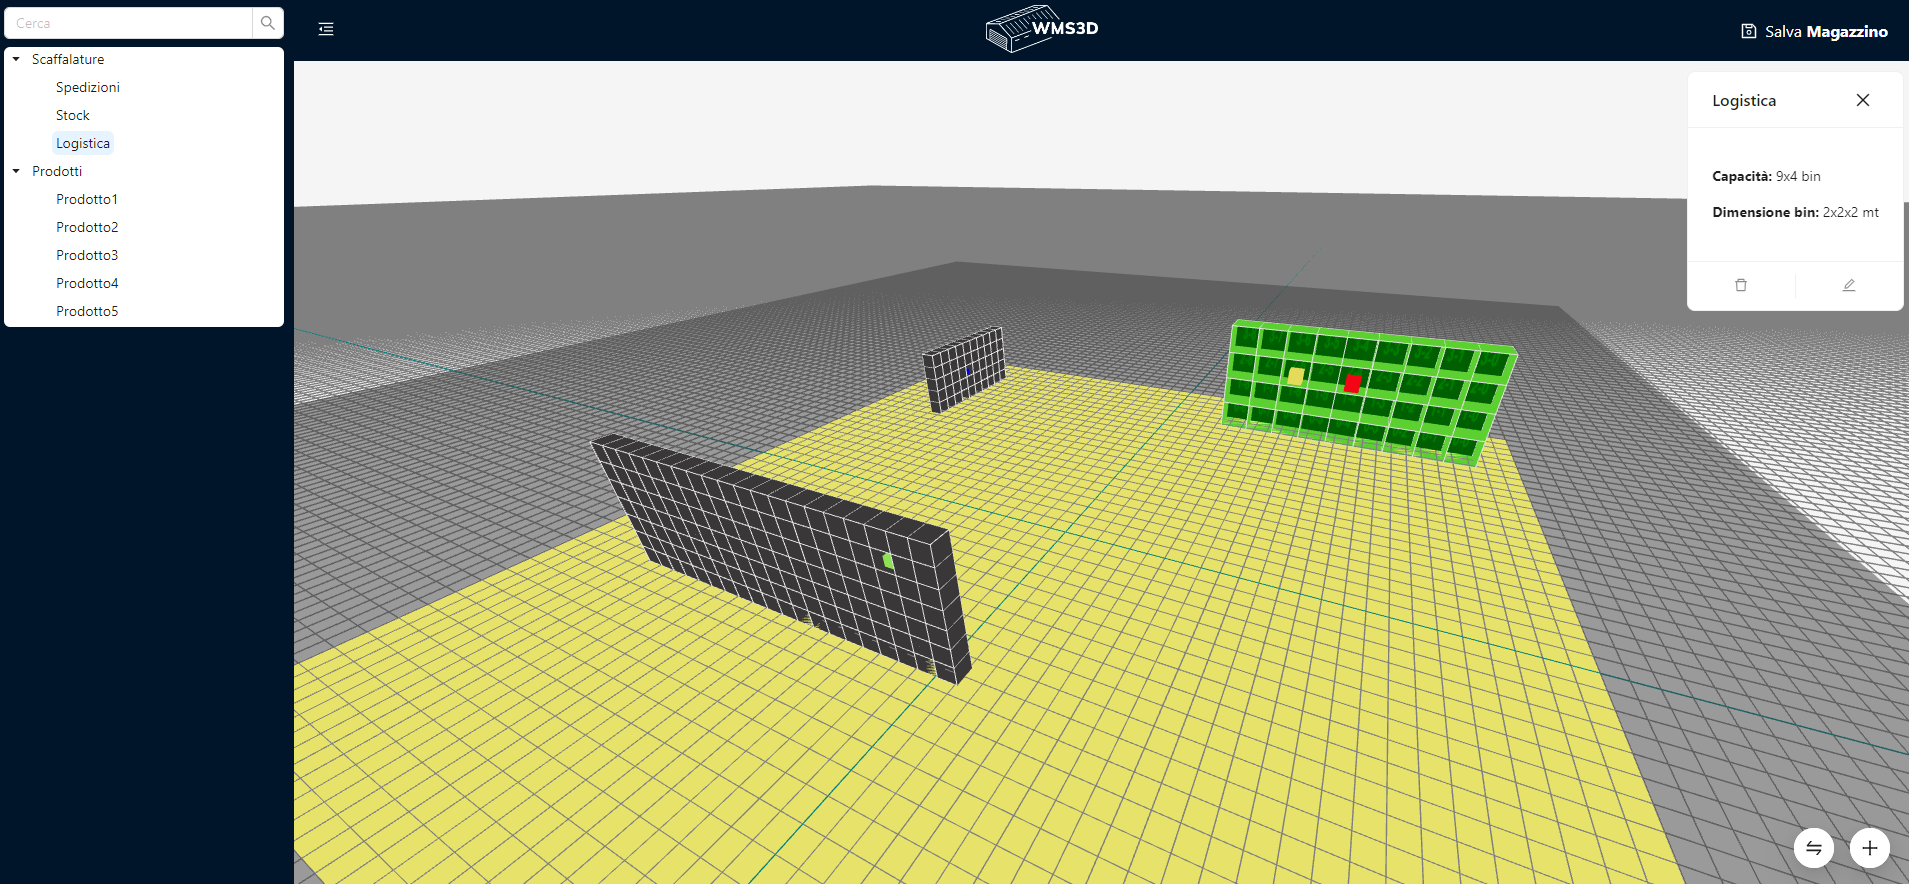
\includegraphics[width=0.8\textwidth]{images/selezione_scaffalatura.png}
                    \caption{Selezione scaffalatura da render 3D}
                \end{figure}
                In caso di selezione di uno specifico bin verrà invece visualizzato: 
                \begin{itemize}
                    \item Lo stato del bin, che può essere: 
                    \begin{enumerate}
                        \item \textbf{Empty}: bin vuoto
                        \item \textbf{Still}: bin occupato da un prodotto 
                        \item \textbf{Outgoing}: bin ancora occupato ma per il prodotto all'interno è stato richiesto lo spostamento
                        \item \textbf{Ingoing}: bin appena occupato da una richiesta di spostamento
                    \end{enumerate}
                    \item Il nome del prodotto eventualmente presente in esso 
                \end{itemize}
                \begin{figure}[h!]
                    \centering
                    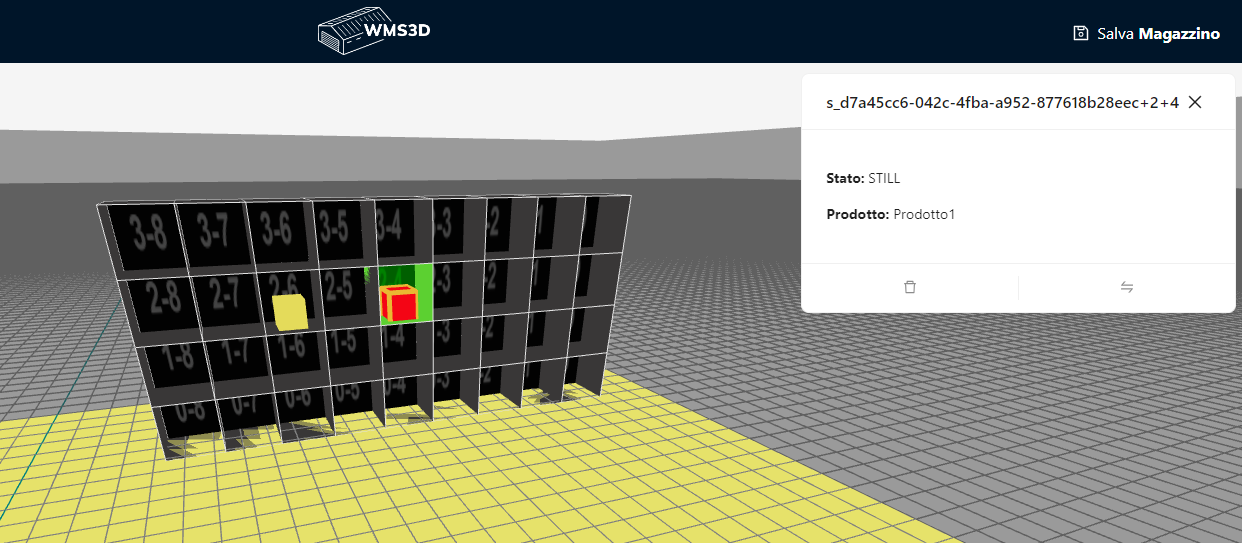
\includegraphics[width=0.8\textwidth]{images/selezione_bin.png}
                    \label{sel_bin}
                    \caption{Selezione bin da render 3D}
                \end{figure}

            \paragraph{Ricerca prodotti in libreria} \label{sec:principale:esplorare:ricerca}
                \noindent All'interno della libreria sarà invece possibile visualizzare l'elenco di tutti i componenti finora creati.\\
                Verranno quindi elencate tutte le scaffalature posizionate all'interno del render e tutti i prodotti creati. Si segnala che \textbf{un prodotto può essere creato
                e non posizionato}. In tal caso sarà quindi elencato in libreria ma sarà non presente sul render 3D.\\
                \begin{figure}[h!]
                    \centering
                    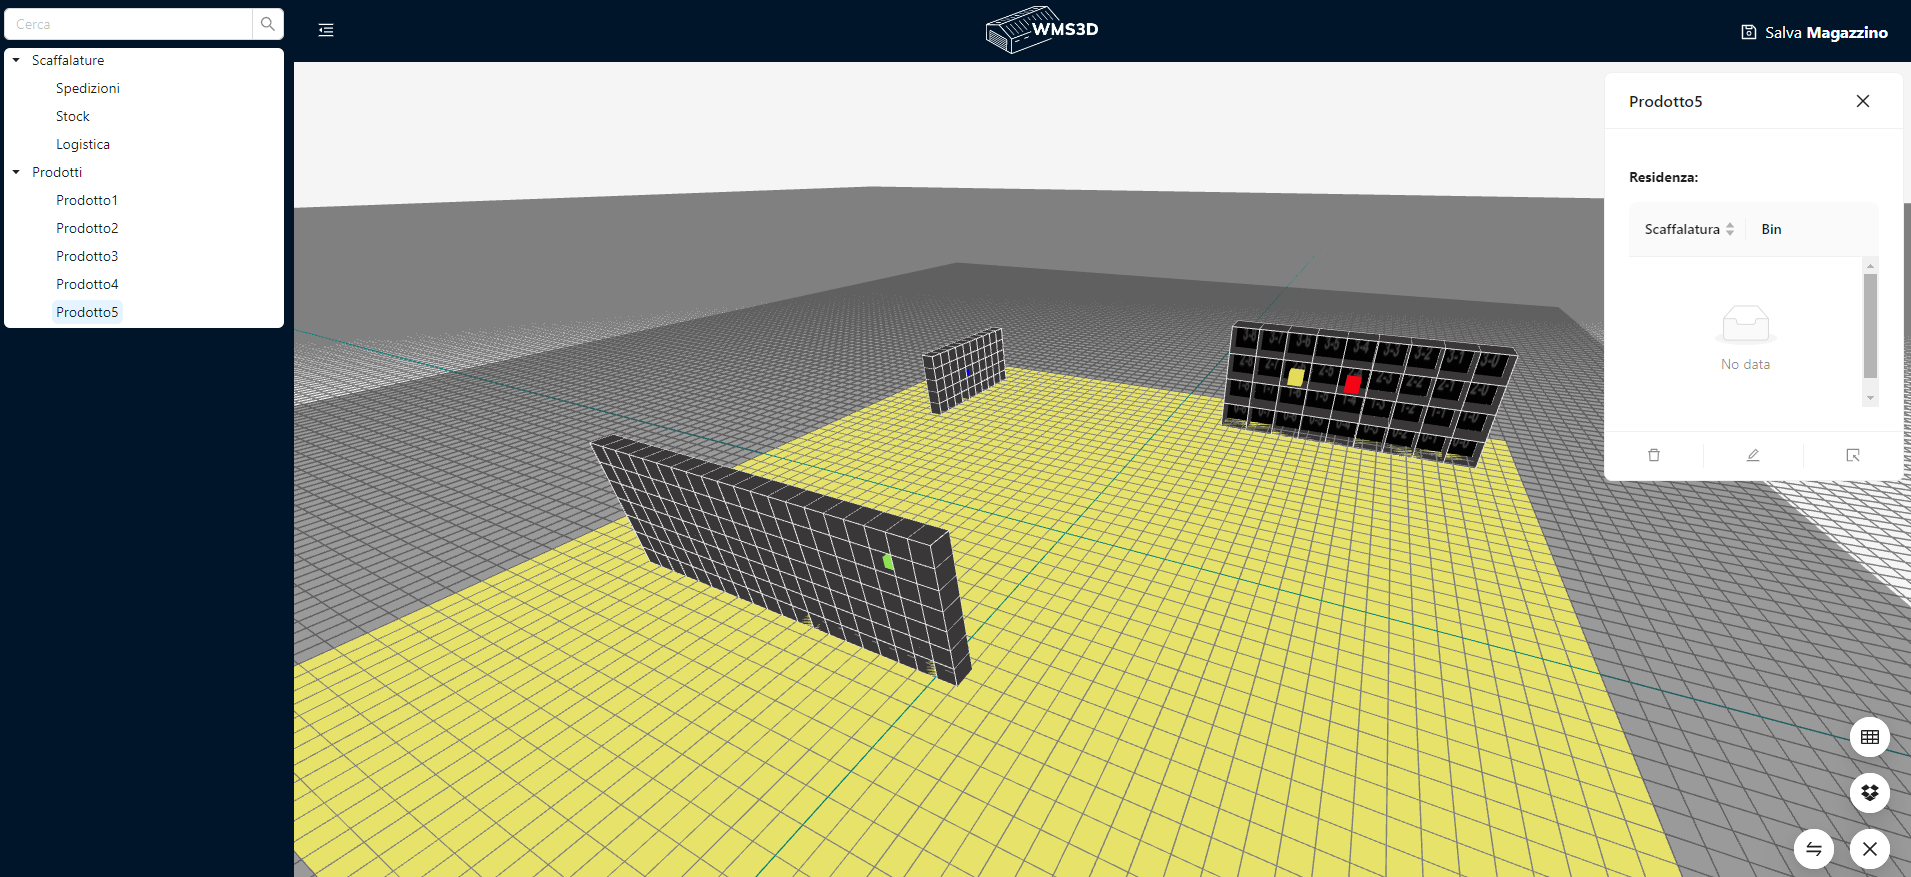
\includegraphics[width=1.0\textwidth]{images/prodotto_no_render.png}
                    \caption{Prodotto aggiunto alla libreria ma non presente sul render}
                \end{figure}
                
                \noindent All'interno della libreria è inoltre presente uno strumento per facilitare la ricerca di uno specifico componente. L'utente, inserendo nell'apposito
                form il nome del componente desiderato, andrà a filtrare il contrnuto della libreria per identificare il prodotto/scaffalatura di interesse. \\\
                \begin{figure}[h!]
                    \centering
                    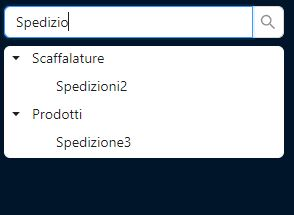
\includegraphics[width=0.4\textwidth]{images/filtro_ricerca.png}
                    \caption{Ricerca da libreria}
                \end{figure}
                
                \noindent Tutti i componenti presenti in libreria sono ovviamente selezionabili, anche in presenza del filtro sopra illustrato. Il risultato della selezione dalla 
                libreria è assolutamente analogo a quello ottenuto attraverso la selezione da render. Verrà quindi evidenziato il prodotto scelto, sia sull'elenco presente in 
                libreria sia sul render 3D, e verrà visualizzato il riquadro con i dettagli del componente. \\
                \begin{figure}[h!]
                    \centering
                    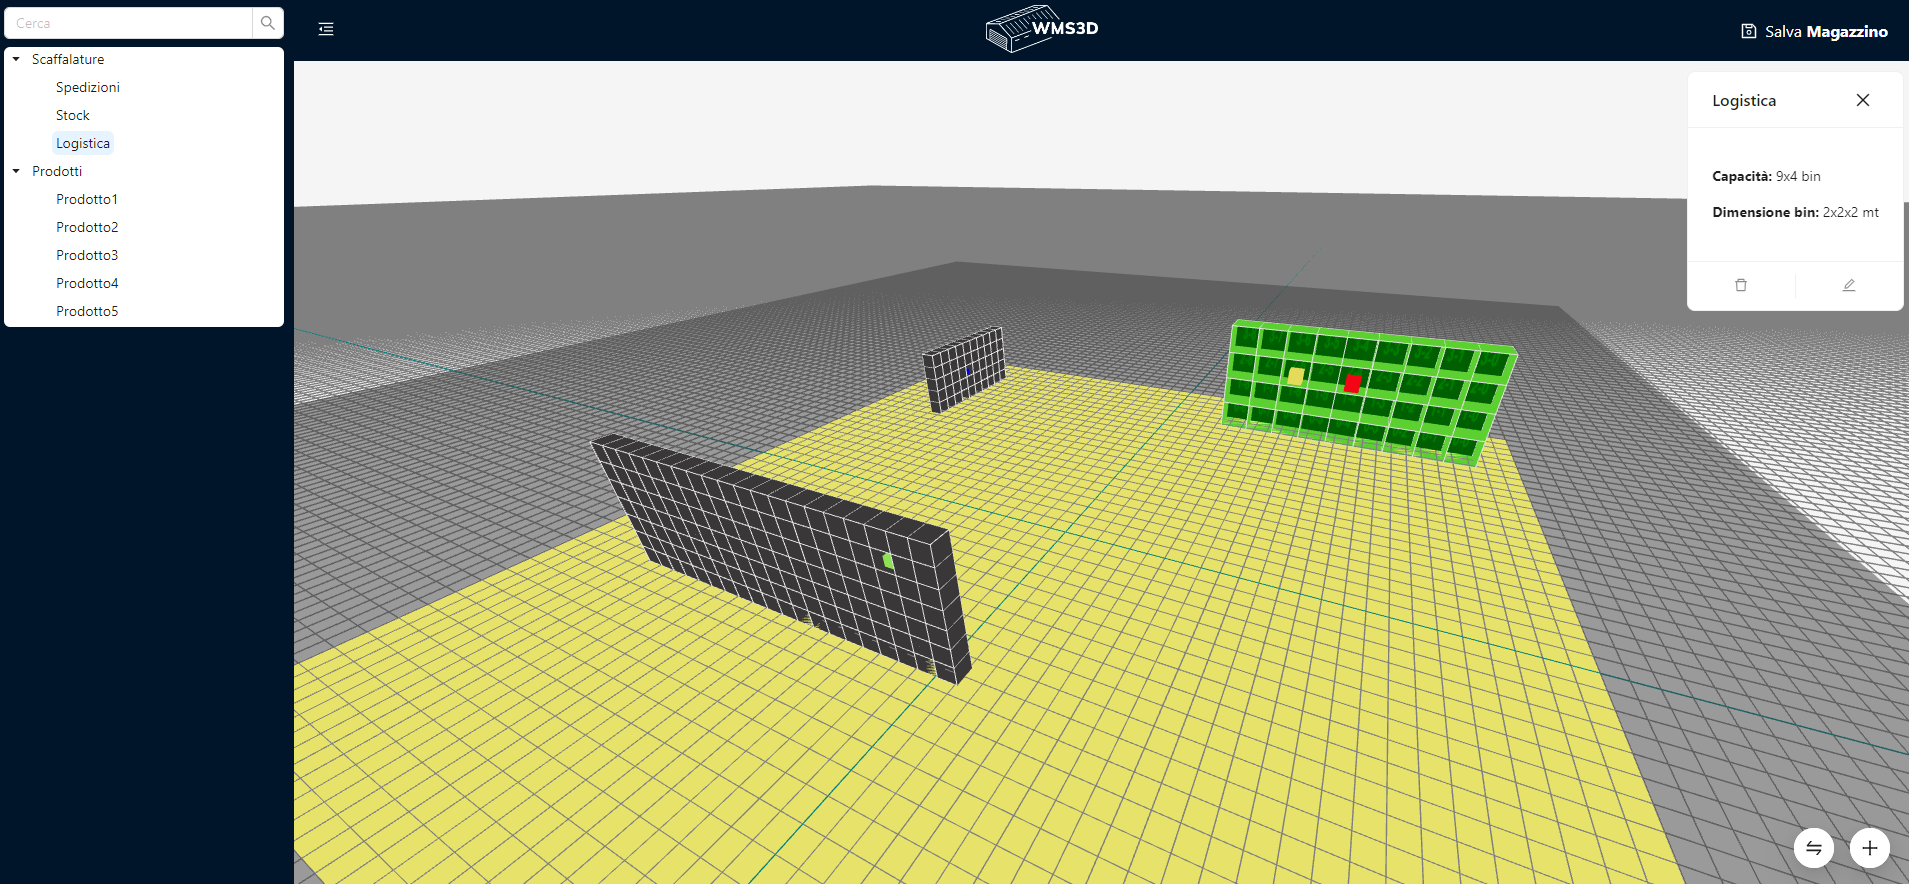
\includegraphics[width=0.8\textwidth]{images/selezione_scaffalatura.png}
                    \caption{Selezione scaffalatura da libreria}
                \end{figure}

    


    \newpage
    \subsection{Scaffalature}\label{sec:scaffalature}
        \subsubsection{Aggiunta scaffalatura}\label{sec:scaffalature:aggiunta}
            Per poter aggiungere una nuova scaffalatura è necessario premere il tasto "+" presente nell'angolo in basso a destra del render 3D.\\
            \begin{figure}[h!]
                \centering
                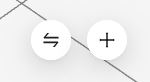
\includegraphics[width=0.3\textwidth]{images/aggiunta_spostamenti.png}
                \caption{Pulsante aggiunta componenti}
            \end{figure}

            \noindent Successivamente, per proseguire, cliccare il tasto relativo alla scaffalatura.\\
            \begin{figure}[h!]
                \centering
                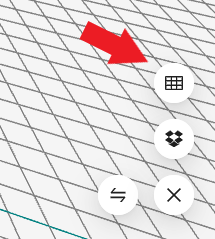
\includegraphics[width=0.3\textwidth]{images/aggiunta_scaffalatura.png}
                \caption{Pulsante aggiunta scaffalatura}
            \end{figure}
            \\
            \noindent Sarà quindi richiesto all'utente di creare la scaffalatura impostando i seguenti campi:\\
            \begin{enumerate}
                \item Il nome che si intende dare alla scaffalatura, attributo univoco della scaffaltura
                \item Dimensione dei singoli bin, espressa in metri
                \item Altezza della scaffalatura, espressa in numero di bin
                \item Larghezza della scaffalatura, espressa in numero di bin 
            \end{enumerate}

            \begin{figure}[h!]
                \centering
                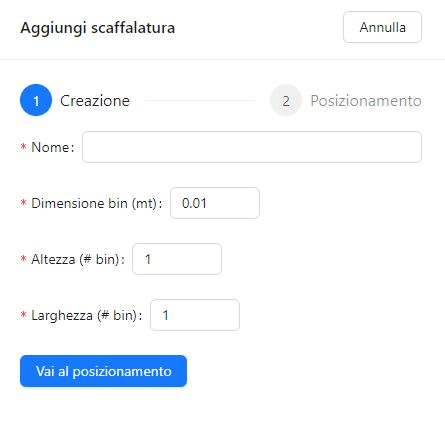
\includegraphics[width=0.4\textwidth]{images/creazione_scaffalatura.png}
                \caption{Form di aggiunta scaffalatura}
            \end{figure}

            \noindent Il passaggio successivo, che completa la creazione, consiste nel posizionare la scaffalatura in uno spazio idoneo del magazzino, in modo tale 
            che non collida con altri elementi presenti nel render e che non oltrepassi i limiti rappresentati dai muri perimetrali. 
            
            \subsubsection{Posizionamento scaffalatura}\label{sec:scaffalature:posizionamento}
            Per riuscire a spostarsi con la scaffalatura sarà necessario utilizzare "l'assistente" al movimento. 
            Sarà infatti presente una traccia per ogni spostamento possibile: spostamento laterale (linea rossa), spostamento in profondità (linea blu), 
            rotazione (linea verde).\\
            Sarà sufficiente quindi selezionare una delle traccie e spostare il cursore verso la direzione designata. In alternativa è possibile spostarsi in tutte e tre 
            le modalità contemporaneamente utilizzando la traccia viola.\\
            \begin{figure}[h!]
                \centering
                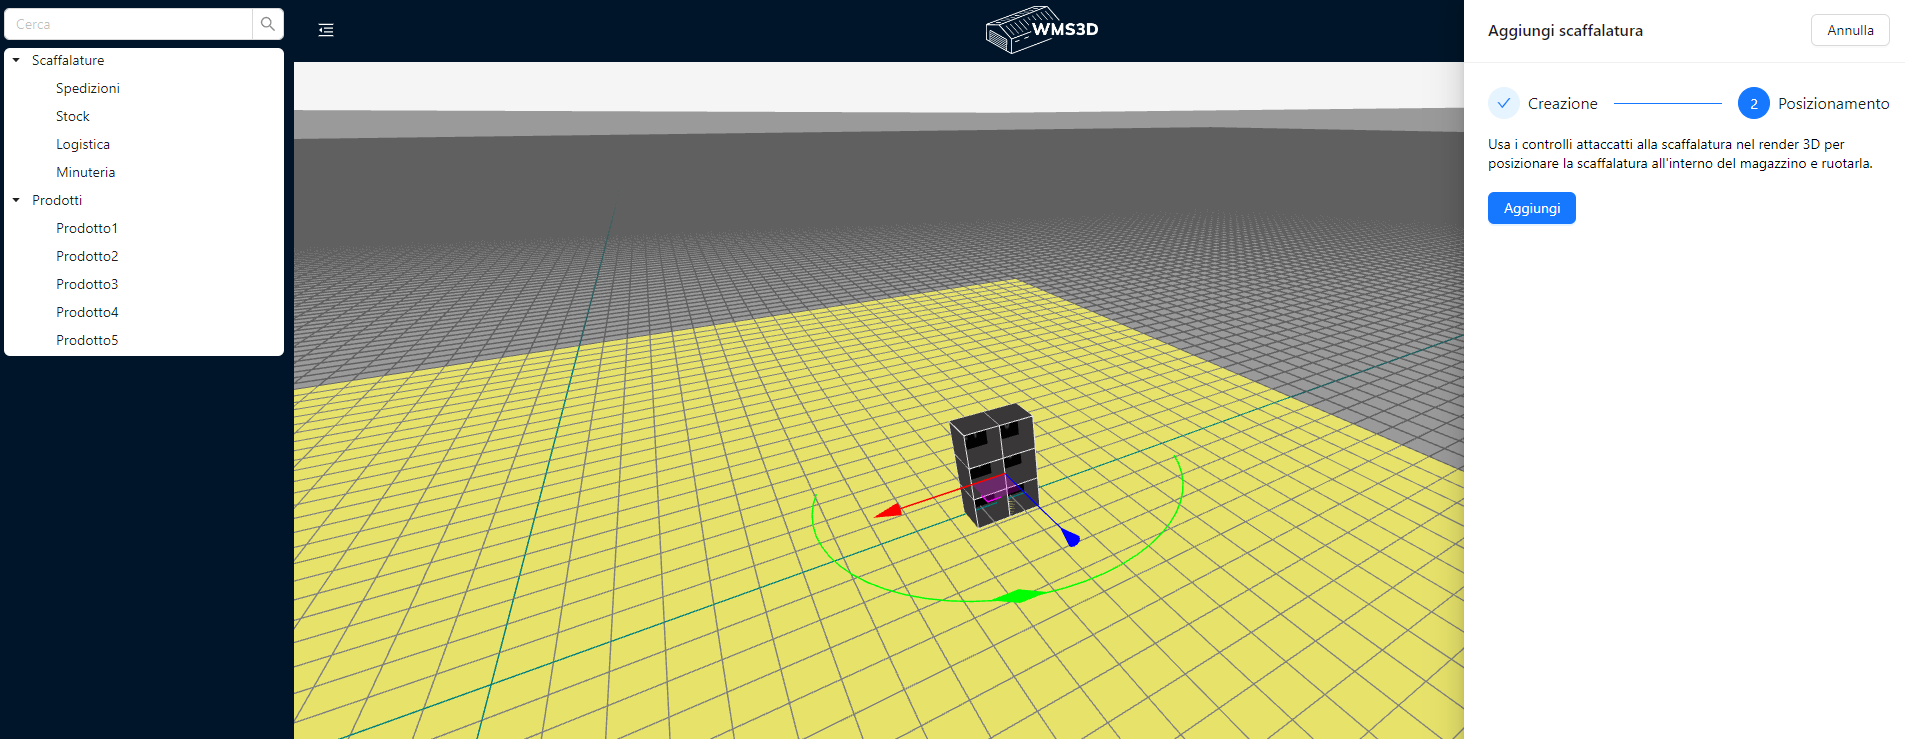
\includegraphics[width=0.8\textwidth]{images/posizionamento.png}
                \caption{Posizionamento scaffalatura}
            \end{figure}
            \\
            \noindent Una volta scelto il punto di posizionamento della scaffalatua completare il processo andando a confermare l'operazione con l'apposito tasto "Aggiungi".  


        \subsubsection{Modifica scaffalatura}\label{sec:scaffalature:modifica}
            Per modificare una scaffalatura esistente sarà sufficiente selezionare la scaffalatura (dal render o dalla libreria) desiderata e premere il pulsante relativo
            all'operazione di interesse presente all'interno della finestra di dettaglio componente. Le operazioni possibili sono l'eliminazione e la modifica. 
            L'eliminazione andrà ovviamente a rimuovere il componente sia dalla libreria che dal render 3D.\\ \\
            Con la modifica invece si entrerà nello stesso processo visto in precedenza con l'\hyperref[sec:scaffalature:aggiunta]{aggiunta scaffalatura} 
            e il \hyperref[sec:scaffalature:posizionamento]{posizionamento}. 
            Sarà quindi possibile cambiare nuovamente tutte le caratteristiche della scaffalatura e/o di cambiarne la posizione nel render.\\ 
            In questo caso però sarà importante valutare la presenza o meno di alcuni prodotti nei vari scaffali. La richiesta di rimozioni dei bin sui quali sono 
            posizionati dei prodotti verrà impedita dal sistema che lancerà l'errore sotto indicato. \\
            \begin{figure}[h!]
                \centering
                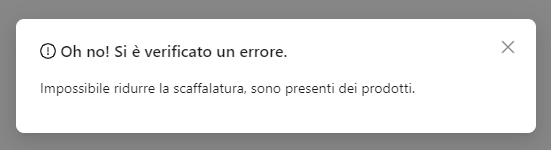
\includegraphics[width=0.4\textwidth]{images/errore_modifica.png}
                \caption{Errore modifica scaffalatura}
            \end{figure}





    \newpage            
    \subsection{Prodotti}\label{sec:prodotti}
        \subsubsection{Aggiunta prodotto}\label{sec:prodotti:aggiunta}
        Per poter aggiungere una nuovo prodotto è necessario premere il tasto "+" presente nell'angolo in basso a destra del render 3D.\\
        \begin{figure}[h!]
            \centering
            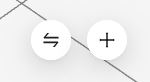
\includegraphics[width=0.3\textwidth]{images/aggiunta_spostamenti.png}
            \caption{Pulsante aggiunta componenti}
        \end{figure}
        
        \noindent Successivamente, per continuare, cliccare il tasto relativo al prodotto.\\
        \begin{figure}[h!]
            \centering
            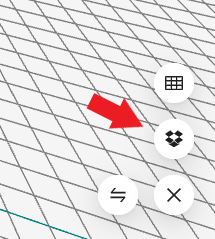
\includegraphics[width=0.3\textwidth]{images/aggiunta_prodotto.png}
            \caption{Pulsante aggiunta prodotto}
        \end{figure}


        \noindent Sarà quindi richiesto all'utente di creare il prodotto impostando i seguenti campi:
        \begin{itemize}
            \item Il nome che si intende dare al prodotto, che sarà univoco
            \item Il colore da assegnare al prodotto
        \end{itemize}
        
        \begin{figure}[h!]
            \centering
            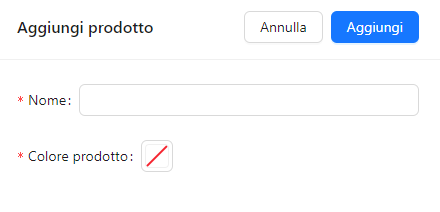
\includegraphics[width=0.6\textwidth]{images/creazione_prodotto.png}
            \caption{Form di aggiunta prodotto}
        \end{figure}

        \subsubsection{Posizionamento prodotto}\label{sec:prodotti:posizionamento}
        \noindent Una volta creato correttamente un prodotto si potrà procedere con il posizionamento dello stesso in uno dei bin liberi delle scaffalature presenti.
        Dopo averlo selezionato dalla libreria sarà quindi possibile, attraveso l'apposito tasto, andare a scegliere il bin di destinazione. 
        \begin{figure}[h!]
            \centering
            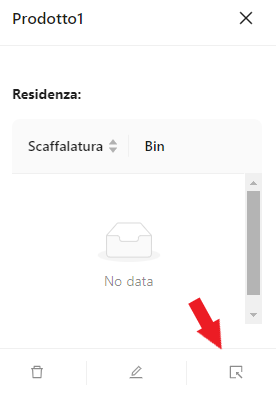
\includegraphics[width=0.3\textwidth]{images/tasto_posizionamento.png}
            \label{riposizionamento}
            \caption{Posizionamento prodotto}
        \end{figure}
        
        \noindent Si aprirà quindi la procedura guidata per andare ad identificare precisamente il bin di destinazione indicando in ordine di presentazione, la
        scaffalatura, il ripiano ed infine la colonna scelta.\\
        \begin{figure}[h!]
            \centering
            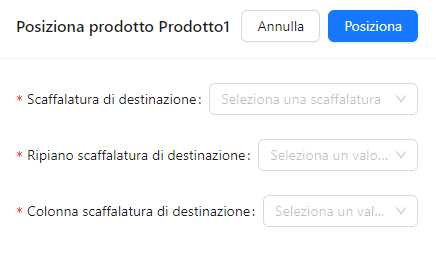
\includegraphics[width=0.4\textwidth]{images/scelta_posizione_prodotto.png}
            \label{destinazione_prodotto}
            \caption{Scelta posizione prodotto}
        \end{figure}
        
        \noindent Anche in questo caso si deve prestare attenzione in quanto i bin già occupati non possono ovviamente essere la destinazione di un secondo prodotto. 
        Tale tentativo segnalerebbe il seguente errore.\\
        \begin{figure}[h!]
            \centering
            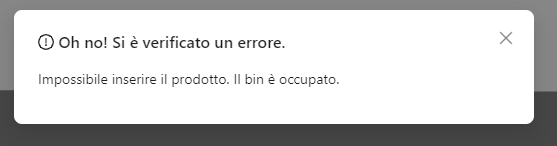
\includegraphics[width=0.4\textwidth]{images/bin_occupato.png}
            \caption{Errore: bin già occupato}
        \end{figure}
        

    \newpage

    \subsubsection{Modifica prodotto}\label{sec:prodotti:modifica}
        Per modificare un prodotto esistente sarà sufficiente selezionarlo dalla libreria e premere il pulsante relativo all'operazione di interesse presente 
        all'interno della finestra di dettaglio componente. Le operazioni possibili sono l'eliminazione e la modifica.  
        L'eliminazione andrà ovviamente a rimuovere il componente sia dalla libreria che dal render 3D (se presente).\\
        
        \noindent Con la modifica invece si entrerà nello stesso processo visto in precedenza con l'\hyperref[sec:prodotti:aggiunta]{aggiunta prodotto}. 
        Sarà quindi possibile cambiare nuovamente il nome e il colore del prodotto scelto. 
       
    \newpage
    \subsection{Movimentazione prodotti}\label{sec:movimento}
        La movimentazione dei prodotti già presenti in render 3D è accessibile in due modalità: 
        \begin{itemize}
            \item Effettuando un nuovo \hyperref[riposizionamento]{riposizionamento del prodotto}. Esattamente come fatto dopo aver selezionato un prodotto da libreria
            \item Premendo l'apposito tasto dopo aver \hyperref[sel_bin]{selezionato il bin} contenente il prodotto da spostare\\
            \begin{figure}[h!]
                \centering
                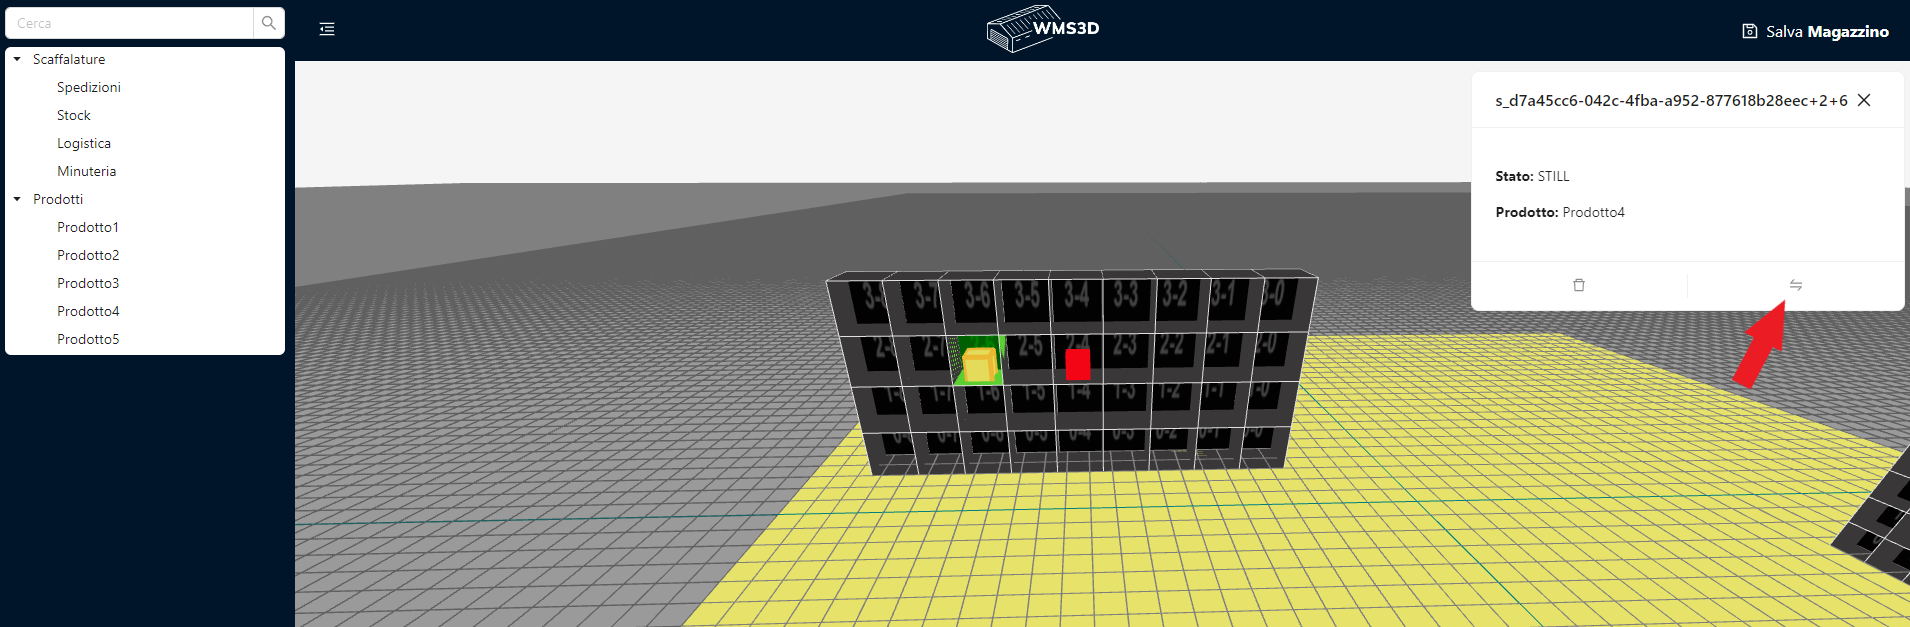
\includegraphics[width=1.0\textwidth]{images/movimentazione.png}
                \caption{Selezione prodotto da libreria per movimentazione}
            \end{figure}
        \end{itemize}
        Entrambe le procedure termineranno con la \hyperref[destinazione_prodotto]{scelta della destinazione} del prodotto. 
        Una volta selezionata correttamente la destinazione del prodotto il sistema andrà ad occupare il bin di arrivo creando un duplicato del prodotto in fase di 
        spostamento. Avremo quindi un bin marchiato "incoming" e un bin marchiato "outcoming". Inoltre il sistema aggiornerà il riquadro dettagli del prodotto andando a 
        inserire anche le coordinate del bin di destinazione.\\
        \begin{figure}[h!]
            \centering
            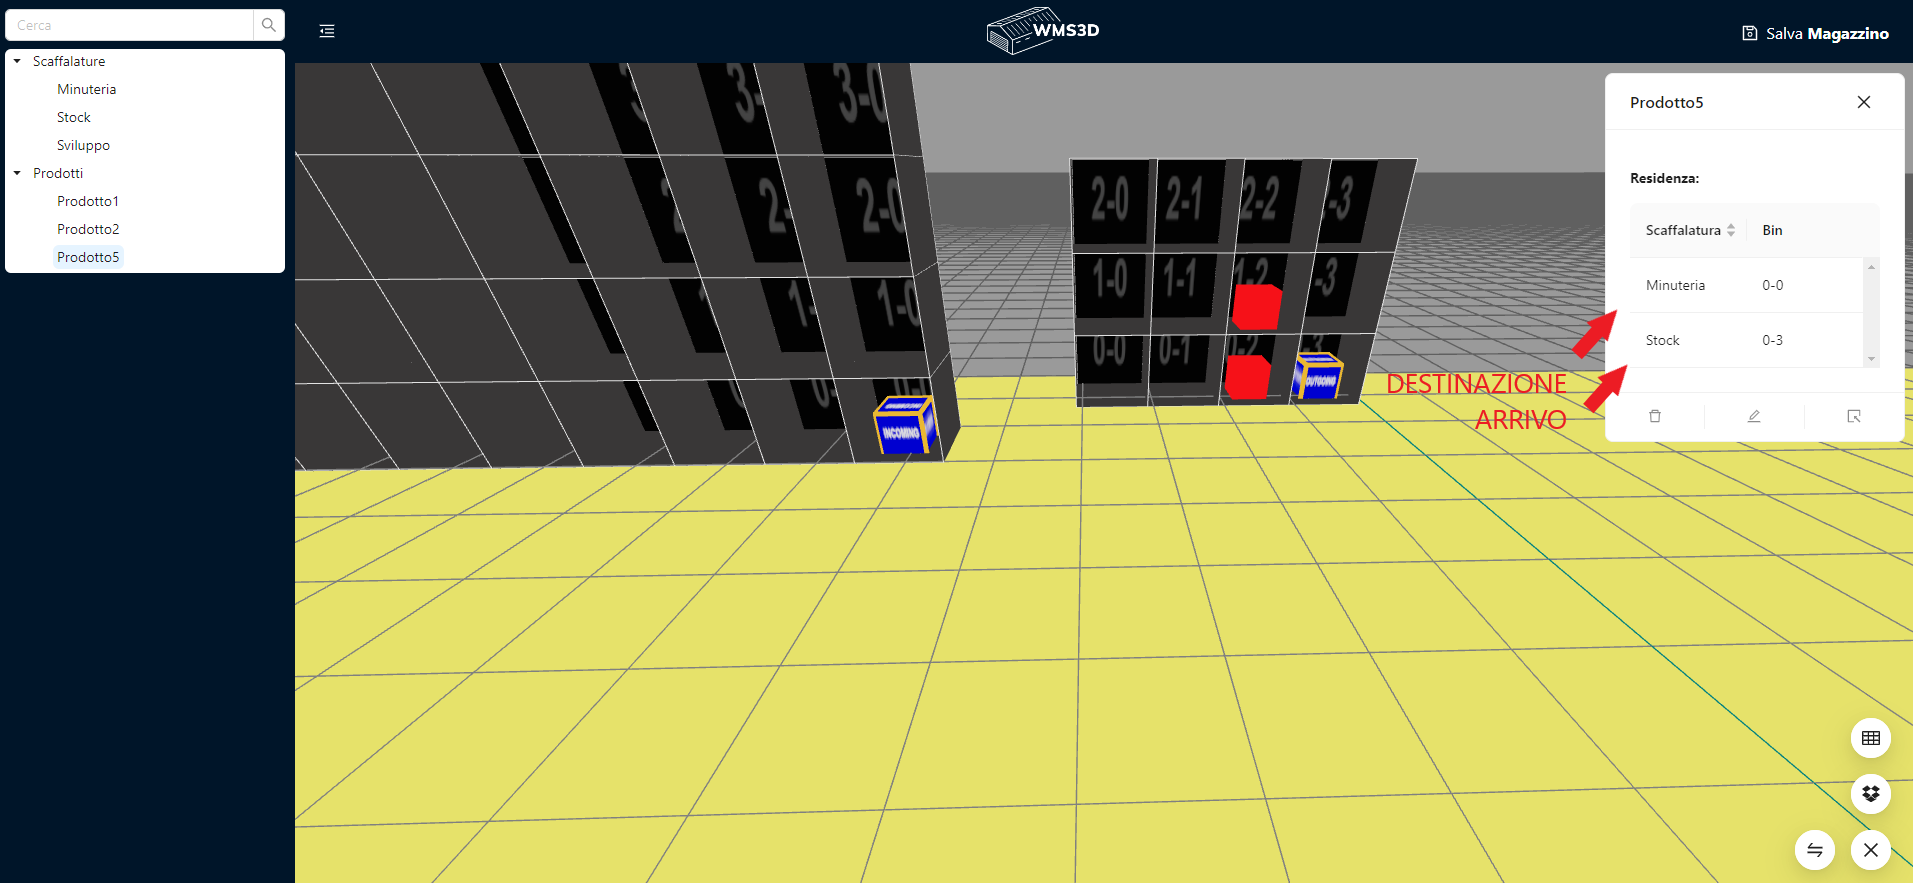
\includegraphics[width=1.0\textwidth]{images/movimento_prodotto.png}
            \caption{Inserimento movimento prodotto}
        \end{figure}\\

        \subsubsection{Lista movimenti} \label{sec:movimento:lista}
        \noindent È possibile inotre consultare la lista dei prodotti attualmente in fase di spostamento selezionado l'apposito bottone in basso a destra nella sezione 3D.
        \begin{figure}[h!]
            \centering
            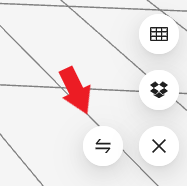
\includegraphics[width=0.2\textwidth]{images/pulsante_lista.png}
            \caption{Pulsante lista movimenti}
        \end{figure}\\
        \noindent Azionandolo si potrà accedere alla lista delle movimentazioni di prodotti in essere in quel istante.
        Inoltre l'utente, attraverso il pulsante "Sollecita risposta" potrà richiedere il completamento di una singola richiesta di spostamento. \\
        \begin{figure}[h!]
            \centering
            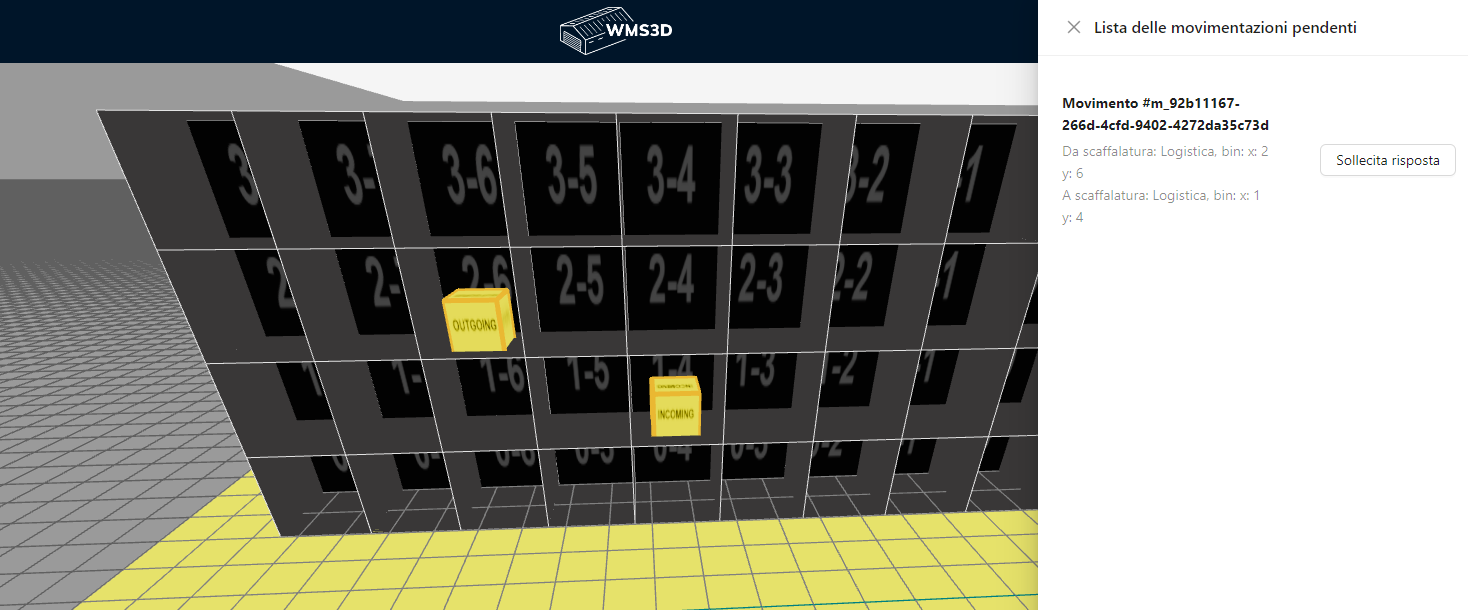
\includegraphics[width=1.0\textwidth]{images/lista_movimenti.png}
            \caption{Lista movimenti}
        \end{figure}\\

        Si ricorda inoltre che tale completamento è dipeso da fattori esterni a tale applicativo e che quindi, per questa versione dell'applicativo, è 
        gestita da un algoritmo autonomo e randomico.
        Potremmo quindi ricevere arbitrariamente un'Approvazione o un rifiuto della richiesta di spostamento. 
        Al termine del processo il componente dublicato (outcoming in caso di rifiuto o incoming in caso di accettazione) verrà rimosso 
        dal render e le scritture adeguate alla decisione presa.\\
        \begin{figure}[h!]
            \centering
            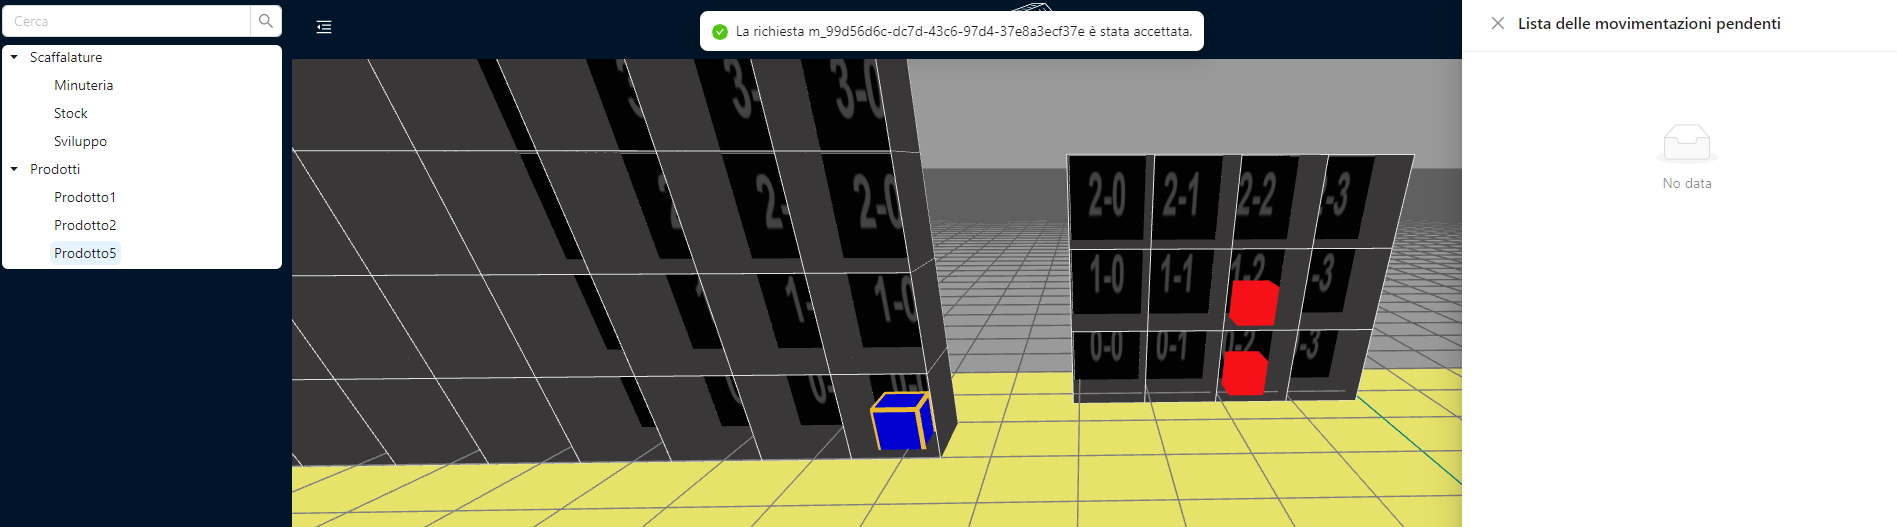
\includegraphics[width=1.0\textwidth]{images/ok_movimento.png}
            \caption{Esempio movimentazione approvata}
        \end{figure}\\


\newpage
%%%%%%%%%%%%%%%%%%%%%%%%%%%%%%%%%%%
% RIFERIMENTI ESTERNI
%%%%%%%%%%%%%%%%%%%%%%%%%%%%%%%%%%%

\section{Riferimenti esterni}\label{sec:riferimenti_esterni}
Per ulteriori chiarimenti sugli argomenti discussi nel documento, si possono consultare i seguenti link esterni:
\begin{itemize}
    \item Capitolato \textbf{Warehouse Management 3D}:\\
    \url{https://www.math.unipd.it/~tullio/IS-1/2023/Progetto/C5.pdf} \textcolor{gray}{\textit{(ultimo accesso 04-05-24)}}
    \item Link alla \textbf{documentazione del gruppo}:\\
    \url{https://avant-garde-software-engineering.github.io/documentazione.html} \textcolor{gray}{\textit{(ultimo accesso 25-04-24)}}
    \item Pagina di installazione al software \textbf{Node.js}:\\
    \url{https://nodejs.org/en/} \textcolor{gray}{\textit{(ultimo accesso 04-05-24)}}
    \item \textbf{Glossario} di progetto: \\
    \url{https://github.com/Avant-Garde-Software-Engineering/WMS3D/blob/main/Documentazione/PB/Esterna/glossario.pdf} \textcolor{gray}{\textit{(ultimo accesso 04-05-24)}}
\end{itemize}